\chapter{Complexation}\label{ch:b1:complexation}

Pour a little ammonia solution into pale blue copper(II) sulfate: a pale
blue precipitate forms at once. Pour more, and the precipitate dissolves
into a solution of a deep, almost ink-like blue. Nothing in the
acid--base or precipitation chapters explains the second step. The
ammonia molecules have bound to the copper ion through their \omterm{def:b1:lewis-resonance-vsepr:lewis}{lone pairs}
and made a new species, a \omterm{def:b1:complexation:complex}{complex}, more stable than the hydroxide and of
a different colour. \omterm{def:b1:complexation:complex}{Complexes} carry oxygen in the blood, hold the metal
in chlorophyll and in vitamin B$_{12}$, soften hard water and dissolve
metals that nothing else will. This chapter treats them as one more
exchange of particles in water, with its own constants and diagrams.

\begin{recall}
\omterm{def:b1:lewis-resonance-vsepr:lewis-acid}{Lewis acids} (electron-pair acceptors), \omterm{def:b1:lewis-resonance-vsepr:lewis-acid}{Lewis bases} (electron-pair donors)
and the \omterm{def:b1:lewis-resonance-vsepr:lewis-acid}{dative bond} were defined in \cref{ch:b1:lewis-resonance-vsepr}.
The \omterm{def:b1:predominant-reaction:predominance}{predominance diagrams} and the predominant-reaction method come from
\cref{ch:b1:predominant-reaction}; the \omterm{def:b1:precipitation:solubility-product}{solubility product} and the
condition of precipitation from \cref{ch:b1:precipitation}.
\end{recall}

\begin{omfigure}
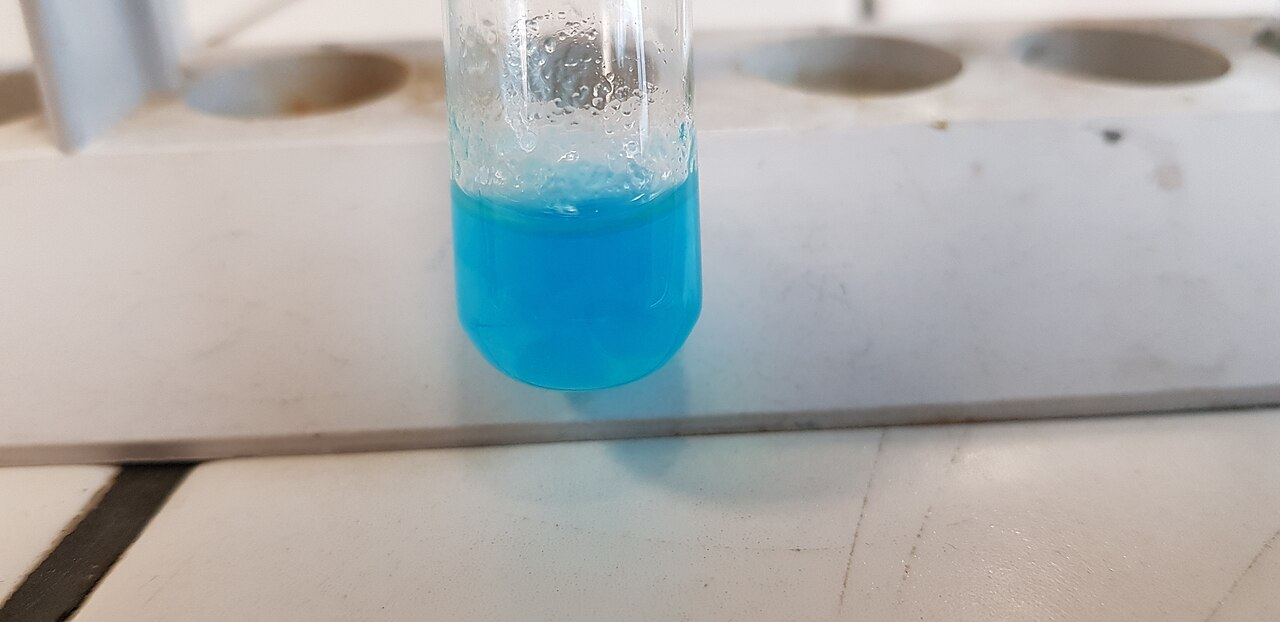
\includegraphics[height=4.2cm]{images/book2/copper-hydroxide.jpg}\hspace{0.6em}%
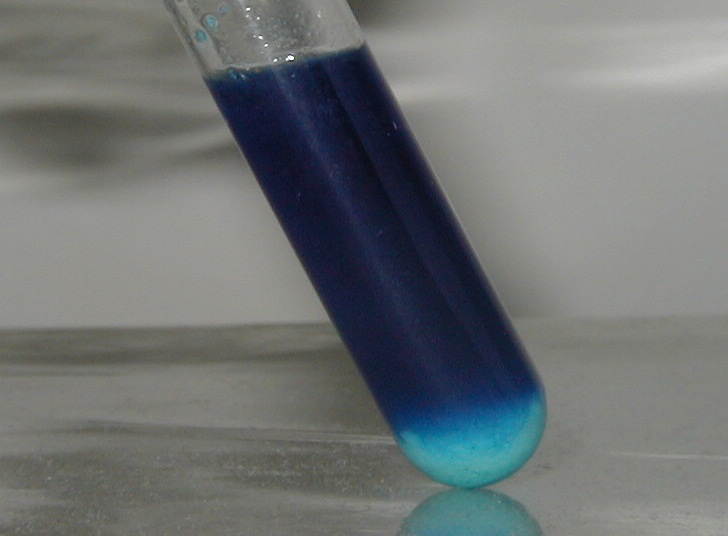
\includegraphics[height=4.2cm]{images/book2/copper-ammine.jpg}

{\small Left: a suspension of pale blue copper(II) hydroxide
(photograph Alvy16, CC BY 4.0). Right: with more ammonia the solid
dissolves into the deep blue tetraamminecopper(II) ion; some undissolved
hydroxide is still at the bottom of the tube (photograph Chemicalinterest,
public domain). Both Wikimedia Commons.}
\end{omfigure}

\section{Complexes and ligands}

\begin{definition}[Complex, central atom, ligand]\label{def:b1:complexation:complex}
A \emph{complex}\index{complex} is a species made of a \emph{central
atom}\index{central atom} or ion, usually a metal cation acting as a
\omterm{def:b1:lewis-resonance-vsepr:lewis-acid}{Lewis acid}, bound by \omterm{def:b1:lewis-resonance-vsepr:lewis-acid}{dative bonds} to molecules or ions acting as \omterm{def:b1:lewis-resonance-vsepr:lewis-acid}{Lewis
bases}, the \emph{ligands}\index{ligand}. Its formula is written in
square brackets, with its total charge: $[\ce{Cu(NH3)4}]^{2+}$,
$[\ce{Fe(CN)6}]^{4-}$, $[\ce{Ag(NH3)2}]^{+}$, $[\ce{FeSCN}]^{2+}$.
\end{definition}

The charge of the \omterm{def:b1:complexation:complex}{complex} is the sum of the charges of the central ion
and of the \omterm{def:b1:complexation:complex}{ligands}: $\mathrm{Fe^{2+}}$ and six \ce{CN-} make
$[\ce{Fe(CN)6}]^{4-}$. A \omterm{def:b1:complexation:complex}{ligand} needs at least one \omterm{def:b1:lewis-resonance-vsepr:lewis}{lone pair}: \ce{NH3},
\ce{H2O}, \ce{OH-}, \ce{Cl-}, \ce{CN-}, \ce{SCN-} (bound through S or N).
Every metal ion in water is in fact already a \omterm{def:b1:complexation:complex}{complex} with water
molecules as \omterm{def:b1:complexation:complex}{ligands}, $[\ce{Cu(H2O)6}]^{2+}$ or $[\ce{Fe(H2O)6}]^{3+}$;
forming another \omterm{def:b1:complexation:complex}{complex} means exchanging those water molecules for other
\omterm{def:b1:complexation:complex}{ligands}, and the water \omterm{def:b1:complexation:complex}{ligands} are left out of the formulas, as \ce{H3O+}
is written for the hydrated proton.

\begin{omfigure}
\begin{tikzpicture}[font=\small, line cap=round]
  % [Ag(NH3)2]+ : linear
  \begin{scope}
    \node (ag) at (0,0) {\ce{Ag}};
    \node (n1) at (-1.2,0) {\ce{H3N}};
    \node (n2) at (1.2,0) {\ce{NH3}};
    \draw[thick] (n1) -- (ag) -- (n2);
    \node at (0,-1.75) {$[\ce{Ag(NH3)2}]^{+}$, linear};
  \end{scope}
  % [Cu(NH3)4]2+ : square plane in perspective
  \begin{scope}[xshift=4.3cm, every node/.style={fill=white, inner sep=1.5pt}]
    \node (cu) at (0,0) {\ce{Cu}};
    \node (a) at (-1.45,-0.5) {\ce{H3N}};
    \node (b) at (1.45,0.5) {\ce{NH3}};
    \node (c) at (0.85,-0.9) {\ce{NH3}};
    \node (d) at (-0.85,0.9) {\ce{H3N}};
    \begin{pgfonlayer}{background}
    \draw[gray, dashed] (a.center) -- (c.center) -- (b.center) -- (d.center) -- cycle;
    \end{pgfonlayer}
    \draw[thick] (cu) -- (a); \draw[thick] (cu) -- (b);
    \draw[thick] (cu) -- (c); \draw[thick] (cu) -- (d);
    \node at (0,-1.75) {$[\ce{Cu(NH3)4}]^{2+}$, square planar};
  \end{scope}
  % [Fe(CN)6]4- : octahedron
  \begin{scope}[xshift=9.2cm, every node/.style={fill=white, inner sep=1.5pt}]
    \node (fe) at (0,0) {\ce{Fe}};
    \node (t) at (0,1.3) {\ce{CN}};
    \node (u) at (0,-1.3) {\ce{CN}};
    \node (l) at (-1.45,-0.45) {\ce{NC}};
    \node (r) at (1.45,0.45) {\ce{CN}};
    \node (f) at (0.8,-0.8) {\ce{CN}};
    \node (k) at (-0.8,0.8) {\ce{NC}};
    \begin{pgfonlayer}{background}
    \draw[gray, dashed] (l.center) -- (f.center) -- (r.center) -- (k.center) -- cycle;
    \end{pgfonlayer}
    \foreach \x in {t,u,l,r,f,k} \draw[thick] (fe) -- (\x);
    \node at (0,-1.75) {$[\ce{Fe(CN)6}]^{4-}$, octahedral};
  \end{scope}
\end{tikzpicture}

{\small Three \omterm{def:b1:complexation:complex}{complexes} and their shapes. Each line is a \omterm{def:b1:lewis-resonance-vsepr:lewis-acid}{dative bond} from
the \omterm{def:b1:lewis-resonance-vsepr:lewis}{lone pair} of the \omterm{def:b1:complexation:complex}{ligand} (the N of ammonia, the C of cyanide) to the
metal ion; dashed lines outline the square of four \omterm{def:b1:complexation:complex}{ligands}. The shapes
of \omterm{def:b1:complexation:complex}{complexes} are explained in the Year~2 volume.}
\end{omfigure}

\begin{definition}[Polydentate ligand, chelate]\label{def:b1:complexation:chelate}
A \omterm{def:b1:complexation:complex}{ligand} that binds the same central ion through several of its atoms at
once is a \emph{polydentate ligand}\index{polydentate ligand}; the
\omterm{def:b1:complexation:complex}{complex} it forms, in which the \omterm{def:b1:complexation:complex}{ligand} closes rings around the metal ion,
is a \emph{chelate}\index{chelate}. Ethylenediamine
\ce{H2N-CH2-CH2-NH2} binds through two N atoms, the oxalate ion
\ce{C2O4^2-} through two O atoms, and the ethylenediaminetetraacetate ion
(\emph{edta}, written \ce{Y^4-}) through two N and four O atoms.
\end{definition}

\begin{omfigure}
\setchemfig{atom sep=1.9em}
\chemfig{N(-[3]-[2]C(=[1]O)-[3]O^{-})(-[5]-[6]C(=[7]O)-[5]O^{-})-[0]-[0]N(-[1]-[2]C(=[3]O)-[1]O^{-})(-[7]-[6]C(=[5]O)-[7]O^{-})}
\hspace{2.2em}
\begin{tikzpicture}[font=\small, baseline=(ca.base)]
  \node[circle, draw, thick, fill=omDef!12, inner sep=1.5pt] (ca) at (0,0) {\ce{Ca}};
  \node (n1) at (-1.15,-0.35) {N};
  \node (n2) at (0.55,-0.6) {N};
  \node (o1) at (0,1.35) {O};
  \node (o2) at (0,-1.35) {O};
  \node (o3) at (1.15,0.35) {O};
  \node (o4) at (-0.55,0.6) {O};
  \foreach \x in {n1,n2,o1,o2,o3,o4} \draw[thick, omDef] (ca) -- (\x);
  \draw[omProp, thick] (n1) .. controls (-0.57,-0.95) .. (n2);
  \draw[omProp, thick] (n1) .. controls (-1.05,0.95) .. (o1);
  \draw[omProp, thick] (n1) .. controls (-1.5,0.25) .. (o4);
  \draw[omProp, thick] (n2) .. controls (0.5,-1.6) .. (o2);
  \draw[omProp, thick] (n2) .. controls (1.5,-0.3) .. (o3);
\end{tikzpicture}

{\small Left: the edta ion \ce{Y^4-}, with its two N atoms and four
carboxylate groups. Right: the calcium--edta \omterm{def:b1:complexation:chelate}{chelate} $[\ce{CaY}]^{2-}$,
schematic: the six donor atoms (blue bonds) sit at the corners of an
octahedron around the ion, the two N atoms side by side, and the carbon
chains of the \omterm{def:b1:complexation:complex}{ligand} (orange) close five rings of five atoms each, the
\omterm{def:b1:complexation:chelate}{chelate} rings.}
\end{omfigure}

The edta ion holds a calcium ion firmly enough to be the reagent of the
titration of water hardness (\cref{ch:b1:titration-methods}).

\section{Formation and dissociation constants}

\begin{definition}[Formation and dissociation constants]\label{def:b1:complexation:formation-constant}
For a central ion M and a \omterm{def:b1:complexation:complex}{ligand} L (charges omitted), the \emph{overall
formation constant}\index{overall formation constant} of
$\mathrm{ML}_n$ is the constant $\beta_n$ of
$\mathrm{M} + n\,\mathrm{L} \rightleftharpoons \mathrm{ML}_n$,
\[
  \beta_n = \frac{[\mathrm{ML}_n]}{[\mathrm{M}][\mathrm{L}]^n} .
\]
The \emph{successive formation constant}\index{successive formation
constant} $K_i$ is that of the addition of one \omterm{def:b1:complexation:complex}{ligand},
$\mathrm{ML}_{i-1} + \mathrm{L} \rightleftharpoons \mathrm{ML}_i$. The
\emph{dissociation constant}\index{dissociation constant} is the
inverse, $K_d = 1/K_i$, and $\mathrm{p}K_d = \log K_i$, so that a
\omterm{def:b1:complexation:complex}{complex}/\omterm{def:b1:complexation:complex}{ligand} pair is described exactly like an acid--base pair, with
the \omterm{def:b1:complexation:complex}{ligand} in place of the proton.
\end{definition}

\begin{proposition}[Overall and successive constants]\label{prop:b1:complexation:beta-k}
$\beta_n = K_1 K_2 \cdots K_n$, that is
$\log\beta_n = \sum_{i=1}^n \log K_i$ and $\log K_i = \log\beta_i -
\log\beta_{i-1}$ (with $\beta_0 = 1$).
\end{proposition}

\begin{proof}
The formation of $\mathrm{ML}_n$ from M is the sum of the $n$ successive
additions; the constant of a sum of reactions is the product of their
constants (\cref{ch:b1:extent-q-and-k}). Directly:
$K_1 K_2\cdots K_n = \frac{[\mathrm{ML}]}{[\mathrm{M}][\mathrm{L}]}
\frac{[\mathrm{ML_2}]}{[\mathrm{ML}][\mathrm{L}]}\cdots
\frac{[\mathrm{ML}_n]}{[\mathrm{ML}_{n-1}][\mathrm{L}]}$, and the
intermediate concentrations cancel.
\end{proof}

\begin{omfigure}
\begin{tabular}{lll}
\hline
\omterm{def:b1:complexation:complex}{complex} & $\log\beta_n$ & $\log K_i$ \\
\hline
$[\ce{Cu(NH3)_n}]^{2+}$, $n = 1$ to 4 & 4.10, 7.51, 10.33, 12.36 & 4.10, 3.41, 2.82, 2.03 \\
$[\ce{Ag(NH3)_n}]^{+}$, $n = 1, 2$ & 3.32, 7.22 & 3.32, 3.90 \\
$[\ce{Zn(OH)4}]^{2-}$ & $\log\beta_4 = 14.45$ & \\
$[\ce{FeSCN}]^{2+}$, $[\ce{FeF}]^{2+}$ & 2.96; 6.85 & \\
$[\ce{CaY}]^{2-}$, $[\ce{MgY}]^{2-}$, $[\ce{NiY}]^{2-}$ & 12.69, 10.90, 20.54 & \\
\hline
\end{tabular}

\smallskip
{\small Formation constants at \qty{25}{\celsius}. The ammine, hydroxo,
thiocyanato and fluoro constants are computed from tabulated standard
Gibbs energies of formation; the edta constants are critically selected
values at zero ionic strength, as are the $\mathrm{p}K_a$ of edta used
below, 2.23, 3.15, 6.80 and 11.24.}
% ledger: dfg:Cu2+_ao, dfg:CuNH32+_ao, dfg:Cu_NH322+_ao, dfg:Cu_NH332+_ao, dfg:Cu_NH342+_ao, dfg:NH3_ao (computed in figdata/bachelor-1/aqueous-constants.py)
% ledger: dfg:Ag+_ao, dfg:AgNH3+_ao, dfg:Ag_NH32+_ao, dfg:Fe3+_ao, dfg:SCN-_ao, dfg:FeSCN2+_ao, dfg:F-_ao, dfg:FeF2+_ao (computed, same script)
% ledger: logb:Ca-edta, logb:Mg-edta, logb:Ni-edta, pka:edta1, pka:edta2, pka:edta3, pka:edta4
\end{omfigure}

The successive constants of the copper ammines decrease, $K_1 > K_2 > K_3
> K_4$: each ammonia molecule added leaves fewer sites and makes the
\omterm{def:b1:complexation:complex}{complex} a little less eager for the next one. This is the usual order.
Silver is an exception: $K_2 > K_1$, with consequences drawn in the
weekend problem.

\section{Predominance in pL}

\begin{definition}[pL scale]\label{def:b1:complexation:pl-diagram}
For a \omterm{def:b1:complexation:complex}{ligand} L, $\mathrm{pL} = -\log[\mathrm{L}]$, where $[\mathrm{L}]$ is
the concentration of the free \omterm{def:b1:complexation:complex}{ligand}. A \emph{pL scale}\index{pL scale}
is an axis of pL on which the domains of predominance of the central ion
and of its \omterm{def:b1:complexation:complex}{complexes} are drawn, as the domains of acids and bases are
drawn on a pH axis.
\end{definition}

\begin{proposition}[Boundaries in pL]\label{prop:b1:complexation:pl-boundaries}
For the pair $\mathrm{ML}_i/\mathrm{ML}_{i-1}$,
\[
  \mathrm{pL} = \log K_i + \log\frac{[\mathrm{ML}_{i-1}]}{[\mathrm{ML}_i]} ,
\]
so that $\mathrm{ML}_{i-1}$ predominates for $\mathrm{pL} > \log K_i$ and
$\mathrm{ML}_i$ for $\mathrm{pL} < \log K_i$. When the $\log K_i$ decrease
with $i$, the diagram is a sequence of domains: $\mathrm{ML}_n$ at small
pL (much \omterm{def:b1:complexation:complex}{ligand}), then $\mathrm{ML}_{n-1}$, down to M at large pL.
\end{proposition}

\begin{proof}
Take the logarithm of $K_i = [\mathrm{ML}_i]/([\mathrm{ML}_{i-1}][\mathrm{L}])$:
$\log K_i = \log\frac{[\mathrm{ML}_i]}{[\mathrm{ML}_{i-1}]} + \mathrm{pL}$.
The two forms are equal at $\mathrm{pL} = \log K_i$, and the ratio moves
by a factor ten per unit of pL. The domain of $\mathrm{ML}_i$ lies between
$\log K_{i+1}$ and $\log K_i$, which exists only if $\log K_{i+1} < \log
K_i$.
\end{proof}

\begin{method}[Drawing a pL diagram]\label{met:b1:complexation:pl-diagram}
\begin{enumerate}
  \item From the $\log\beta_n$, compute the successive $\log K_i$.
  \item If they decrease, place each at its boundary on the pL axis: the
        \omterm{def:b1:complexation:complex}{complex} with the most \omterm{def:b1:complexation:complex}{ligands} on the left (small pL), the free
        ion on the right.
  \item If some $\log K_{i+1} > \log K_i$, the \omterm{def:b1:complexation:complex}{complex} $\mathrm{ML}_i$ has
        no domain: it reacts with itself into $\mathrm{ML}_{i-1}$ and
        $\mathrm{ML}_{i+1}$. Remove it and draw a single boundary between
        $\mathrm{ML}_{i-1}$ and $\mathrm{ML}_{i+1}$ at
        $\frac12(\log K_i + \log K_{i+1})$.
\end{enumerate}
\end{method}

\begin{omfigure}
\begin{tikzpicture}
\begin{axis}[
  width=0.78\linewidth, height=5.2cm, xmin=0, xmax=7, ymin=0, ymax=1.05,
  axis x line=bottom, axis y line=left, xlabel={$\mathrm{pNH_3}$},
  ylabel={fraction of copper},
  tick label style={font=\small}, label style={font=\small}]
\addplot[omThm, thick] table[x=pL, y=M] {figdata/out/bachelor-1-ammine-distribution-copper.dat};
\addplot[omProp, thick] table[x=pL, y=ML] {figdata/out/bachelor-1-ammine-distribution-copper.dat};
\addplot[omMeth, thick] table[x=pL, y=ML2] {figdata/out/bachelor-1-ammine-distribution-copper.dat};
\addplot[black!60, thick] table[x=pL, y=ML3] {figdata/out/bachelor-1-ammine-distribution-copper.dat};
\addplot[omDef, very thick] table[x=pL, y=ML4] {figdata/out/bachelor-1-ammine-distribution-copper.dat};
\node[omDef, font=\small, anchor=west] at (axis cs:0.15,0.78) {$n = 4$};
\node[black!60, font=\small] at (axis cs:2.42,0.63) {3};
\node[omMeth, font=\small] at (axis cs:3.12,0.55) {2};
\node[omProp, font=\small] at (axis cs:3.76,0.58) {1};
\node[omThm, font=\small, anchor=east] at (axis cs:6.9,0.84) {\ce{Cu^2+}};
\end{axis}
\end{tikzpicture}

\begin{tikzpicture}[font=\small, x=1.25cm]
  \draw[->, thick] (0,0) -- (7.2,0) node[right] {$\mathrm{pNH_3}$};
  \foreach \x/\l in {2.03/2.03, 2.82/2.82, 3.41/3.41, 4.10/4.10}
    \draw (\x,0.12) -- (\x,-0.12) node[below] {\l};
  \node[above] at (1.0,0.08) {$[\ce{Cu(NH3)4}]^{2+}$};
  \node[above, font=\scriptsize] at (2.42,0.08) {3};
  \node[above, font=\scriptsize] at (3.12,0.08) {2};
  \node[above, font=\scriptsize] at (3.76,0.08) {1};
  \node[above] at (5.6,0.08) {\ce{Cu^2+}};
  \begin{scope}[yshift=-1.25cm]
  \draw[->, thick] (0,0) -- (7.2,0) node[right] {$\mathrm{pNH_3}$};
  \draw (3.61,0.12) -- (3.61,-0.12) node[below] {3.61};
  \draw[dotted] (3.32,0.3) -- (3.32,-0.1); \draw[dotted] (3.90,0.3) -- (3.90,-0.1);
  \node[above] at (1.6,0.08) {$[\ce{Ag(NH3)2}]^{+}$};
  \node[above] at (5.4,0.08) {\ce{Ag+}};
  \end{scope}
\end{tikzpicture}

{\small Top: fractions of copper(II) present as \ce{Cu^2+} and as
$[\ce{Cu(NH3)_n}]^{2+}$ ($n = 1$ to 4) against $\mathrm{pNH_3}$. Middle:
the \omterm{def:b1:predominant-reaction:predominance}{predominance diagram} of the copper ammines, boundaries at the
$\log K_i$. Bottom: silver, where $\log K_2 = 3.90 > \log K_1 = 3.32$
(dotted): $[\ce{AgNH3}]^{+}$ has no domain and a single boundary lies at
$\frac12\log\beta_2 = 3.61$.}
\end{omfigure}

\begin{example}[Copper in \texorpdfstring{\qty{0.010}{mol/L}}{0.010 mol/L} ammonia]\label{ex:b1:complexation:cu}
At free $[\ce{NH3}] = \qty{0.010}{mol/L}$, $\mathrm{pNH_3} = 2.0$ lies in
the domain of $[\ce{Cu(NH3)3}]^{2+}$ but close to the boundary 2.03 with
$[\ce{Cu(NH3)4}]^{2+}$: the two are nearly equal. The fractions are
proportional to $\beta_n[\ce{NH3}]^n = 10^{\log\beta_n - 2n}$, that is
$1 : 10^{2.10} : 10^{3.51} : 10^{4.33} : 10^{4.36}$, so \qty{48}{\percent} of
$[\ce{Cu(NH3)4}]^{2+}$, \qty{45}{\percent} of $[\ce{Cu(NH3)3}]^{2+}$,
\qty{7}{\percent} of $[\ce{Cu(NH3)2}]^{2+}$ and almost no free \ce{Cu^2+}.
\end{example}

\section{Competitions}

A \omterm{def:b1:complexation:complex}{ligand} can be claimed by two metal ions, a metal ion by two \omterm{def:b1:complexation:complex}{ligands},
and both are also engaged in precipitation and acid--base equilibria.
Each competition is one more reaction whose constant combines the
constants already known; the predominant-reaction method of
\cref{ch:b1:predominant-reaction} then applies unchanged.

\begin{example}[Two ligands for iron(III)]\label{ex:b1:complexation:scn-f}
A drop of thiocyanate in an iron(III) solution gives the blood-red
$[\ce{FeSCN}]^{2+}$; fluoride ions decolourise it:
\[
  [\ce{FeSCN}]^{2+} + \ce{F-} \rightleftharpoons [\ce{FeF}]^{2+} + \ce{SCN-},
  \qquad K = \frac{\beta(\ce{FeF})}{\beta(\ce{FeSCN})} = 10^{6.85 - 2.96} =
  10^{3.89} .
\]
The stronger \omterm{def:b1:complexation:complex}{complex} (larger $\beta$) takes the metal ion, exactly as the
stronger acid gives its proton to the stronger base.
\end{example}

\begin{proposition}[Complexation against precipitation]\label{prop:b1:complexation:competition-precipitation}
A solid MX dissolves in a \omterm{def:b1:complexation:complex}{ligand} L by
$\mathrm{MX(s)} + n\,\mathrm{L} \rightleftharpoons \mathrm{ML}_n + \mathrm{X}$,
of constant $K = \beta_n K_s$. If the \omterm{def:b1:complexation:complex}{complex} is the only form of M in
solution and the free \omterm{def:b1:complexation:complex}{ligand} concentration is $[\mathrm{L}]$, the
\omterm{def:b1:precipitation:solubility}{solubility} is $s = \sqrt{K}\,[\mathrm{L}]^{n/2}$.
\end{proposition}

\begin{proof}
The reaction is the sum of the dissolution (constant $K_s$) and of the
formation of $\mathrm{ML}_n$ ($\beta_n$). At saturation $[\mathrm{ML}_n]
= [\mathrm{X}] = s$ and $K = s^2/[\mathrm{L}]^n$.
\end{proof}

\begin{method}[Dissolving a precipitate by complexation]\label{met:b1:complexation:dissolve-precipitate}
\begin{enumerate}
  \item Write the dissolution reaction into the \omterm{def:b1:complexation:complex}{complex} and compute
        $K = \beta_n K_s$.
  \item If $K$ is large, the dissolution is \omterm{def:b1:extent-q-and-k:quantitative}{quantitative} as long as
        enough \omterm{def:b1:complexation:complex}{ligand} is present; if it is small, compute the free \omterm{def:b1:complexation:complex}{ligand}
        concentration needed for the amount of solid to dissolve:
        $[\mathrm{L}]^n = s^2/K$.
  \item Add the \omterm{def:b1:complexation:complex}{ligand} bound in the \omterm{def:b1:complexation:complex}{complex}, $n s$, to obtain the total
        \omterm{def:b1:complexation:complex}{ligand} to introduce.
  \item Check that the free metal ion is negligible: $[\mathrm{M}] = K_s/s
        \ll s$.
\end{enumerate}
\end{method}

With ammonia, silver chloride ($K = 10^{7.22 - 9.75} = 10^{-2.53}$)
dissolves in moderately concentrated solution while silver iodide
($K = 10^{-8.85}$) does not: the weekend problem uses this to tell the
halides apart.

\begin{proposition}[Complexation against acidity]\label{prop:b1:complexation:ligand-acidity}
If the \omterm{def:b1:complexation:complex}{ligand} is a base $\mathrm{L}$ of an acid $\mathrm{HL}$ (and
possibly more protonated forms), only the fraction $[\mathrm{L}]/c_L =
1/\alpha$ of the \omterm{def:b1:complexation:complex}{ligand} not bound to the metal is available, with
\[
  \alpha = 1 + \frac{[\ce{H3O+}]}{K_{an}} + \frac{[\ce{H3O+}]^2}{K_{an}K_{a(n-1)}}
  + \cdots
\]
($K_{an}$ the last \omterm{def:b1:predominant-reaction:acidity-constant}{acidity constant}). At a fixed pH the complexation then
behaves as if its constant were the \emph{conditional} constant
$\beta' = \beta/\alpha$, smaller the lower the pH.
\end{proposition}

\begin{proof}
The \omterm{def:b1:complexation:complex}{ligand} not bound to the metal is shared among L, HL, \ce{H2L} and
so on, with $[\mathrm{HL}] = [\mathrm{L}][\ce{H3O+}]/K_{an}$ and similar
relations for the next forms (\cref{ch:b1:predominant-reaction}). Summing gives $c_L = \alpha[\mathrm{L}]$,
and $\beta = [\mathrm{ML}]/([\mathrm{M}][\mathrm{L}]) =
\alpha[\mathrm{ML}]/([\mathrm{M}]c_L)$, so $[\mathrm{ML}]/([\mathrm{M}]c_L)
= \beta/\alpha$.
\end{proof}

For edta at pH 10, $\alpha = 1 + 10^{11.24 - 10} + 10^{11.24 + 6.80 - 20}
= 18.4$, so the calcium \omterm{def:b1:complexation:complex}{complex} keeps $\log\beta' = 12.69 - 1.26 = 11.43$;
at pH 7 it falls to 8.24 (\cref{exo:b1:complexation:9}). This is why a
titration of calcium with edta is run in an ammonia buffer at pH 10.
Ammonia, too, is a base: in acid it becomes \ce{NH4+}, which has no \omterm{def:b1:lewis-resonance-vsepr:lewis}{lone
pair}, and the ammine \omterm{def:b1:complexation:complex}{complexes} fall apart. Adding nitric acid to
$[\ce{Ag(NH3)2}]^{+}$ in the presence of chloride brings back the white
precipitate of silver chloride.

Photographic fixers do the same with another \omterm{def:b1:complexation:complex}{ligand} of the silver ion,
the thiosulfate ion \ce{S2O3^2-}: they dissolve the silver halide that
light has not touched, so that the picture no longer darkens. Its
constants are not among the data of this volume; ammonia shows the same
chemistry with silver chloride.

\section{Exercises}

\begin{exercise}[$\star$]\label{exo:b1:complexation:1}
For each \omterm{def:b1:complexation:complex}{complex} give the central ion, its charge, the \omterm{def:b1:complexation:complex}{ligands} and the
atom through which each \omterm{def:b1:complexation:complex}{ligand} binds: $[\ce{Cu(NH3)4}]^{2+}$,
$[\ce{Fe(CN)6}]^{4-}$, $[\ce{Fe(CN)6}]^{3-}$, $[\ce{Ag(NH3)2}]^{+}$,
$[\ce{FeSCN}]^{2+}$, $[\ce{Zn(OH)4}]^{2-}$, $[\ce{CaY}]^{2-}$.
\end{exercise}

\begin{exercise}[$\star$]\label{exo:b1:complexation:2}
From the $\log\beta_n$ of the copper ammines, compute the four $\log K_i$
and the four $\mathrm{p}K_d$. Write the dissociation reaction to which
the last $\mathrm{p}K_d$ refers.
\end{exercise}

\begin{exercise}[$\star$]\label{exo:b1:complexation:3}
Draw the pL diagram of the copper ammines. Which copper species
predominates at $[\ce{NH3}] = 1.0$, \num{3.2e-3}, \num{3.2e-4} and
\qty{1.0e-5}{mol/L}?
\end{exercise}

\begin{exercise}[$\star$]\label{exo:b1:complexation:4}
A solution contains iron(III) at \qty{1.0e-3}{mol/L} and thiocyanate at
\qty{0.10}{mol/L}. Neglecting the thiocyanate bound, what fraction of
the iron is present as $[\ce{FeSCN}]^{2+}$?
\end{exercise}

\begin{exercise}[$\star\star$]\label{exo:b1:complexation:5}
Prove that in a solution of a metal ion M and its \omterm{def:b1:complexation:complex}{complexes}
$\mathrm{ML}_n$, the fraction of $\mathrm{ML}_n$ is
$\beta_n[\mathrm{L}]^n / \sum_{k} \beta_k[\mathrm{L}]^k$. Show that,
if only $\mathrm{ML}_{i-1}$, $\mathrm{ML}_i$ and $\mathrm{ML}_{i+1}$ are
present in significant amounts, the fraction of $\mathrm{ML}_i$ is
largest where $[\mathrm{ML}_{i-1}] = [\mathrm{ML}_{i+1}]$, at
$\mathrm{pL} = \frac12(\log K_i + \log K_{i+1})$, and compute this pNH3
for $[\ce{Cu(NH3)2}]^{2+}$.
\end{exercise}

\begin{exercise}[$\star\star$]\label{exo:b1:complexation:6}
To the red solution of \cref{exo:b1:complexation:4}, sodium fluoride is
added until $[\ce{F-}] = \qty{0.010}{mol/L}$ (free). Compute the constant
of the exchange of \omterm{def:b1:complexation:complex}{ligands} and the ratio $[\ce{FeF^2+}]/[\ce{FeSCN^2+}]$.
What does one see?
\end{exercise}

\begin{exercise}[$\star\star$]\label{exo:b1:complexation:7}
Calcium ions are added to a solution of $[\ce{MgY}]^{2-}$, in equal
amount. Write the exchange reaction, compute its constant and the
fraction of magnesium set free.
\end{exercise}

\begin{exercise}[$\star\star$]\label{exo:b1:complexation:8}
Silver oxide \ce{Ag2O} is a brown solid: \ce{Ag2O(s) + H2O <=> 2Ag+ + 2OH-}
has $\mathrm{p}K = 15.43$. Write its dissolution in ammonia into
$[\ce{Ag(NH3)2}]^{+}$, compute the constant, and explain why the brown
precipitate formed by a little ammonia in silver nitrate dissolves in
more ammonia.
\end{exercise}

\begin{exercise}[$\star\star$]\label{exo:b1:complexation:9}
Compute $\alpha$ and the conditional constant $\log\beta'$ of $[\ce{CaY}]^{2-}$
at pH 10 and at pH 7 (\cref{prop:b1:complexation:ligand-acidity}). Why is
a titration of calcium by edta impossible in neutral solution if a
conditional constant of at least $10^{10}$ is required?
\end{exercise}

\begin{exercise}[$\star\star\star$]\label{exo:b1:complexation:10}
Copper(II) oxide \ce{CuO} is the solid that copper(II) hydroxide turns into
on standing; \ce{CuO(s) + H2O <=> Cu^2+ + 2OH-} has $\mathrm{p}K = 20.64$.
\begin{enumerate}
  \item Write the dissolution of \ce{CuO} in ammonia into
        $[\ce{Cu(NH3)4}]^{2+}$ and compute its constant.
  \item In \qty{1.0}{mol/L} ammonia alone, the pH is fixed by ammonia
        ($\mathrm{p}K_a(\ce{NH4+}) = 9.25$). Compute the pH and the
        concentration of copper dissolved.
  \item Same question in a buffer of ammonia and ammonium chloride, both
        at \qty{1.0}{mol/L}. Conclude.
\end{enumerate}
\end{exercise}

\begin{exercise}[$\star\star\star$]\label{exo:b1:complexation:11}
Silver and ammonia.
\begin{enumerate}
  \item Show that $[\ce{AgNH3}]^{+}$ reacts with itself,
        \ce{2[AgNH3]+ <=> Ag+ + [Ag(NH3)2]+}, and compute the constant.
  \item Compute the largest fraction of silver ever present as
        $[\ce{AgNH3}]^{+}$, and the pNH3 where it occurs.
\end{enumerate}
\end{exercise}

\begin{exercise}[$\star\star\star$]\label{exo:b1:complexation:12}
A solution of edta, \qty{0.10}{mol/L} of \ce{Y^4-} at high pH, is used to
dissolve calcium carbonate scale.
\begin{enumerate}
  \item Write the reaction and compute its constant.
  \item What mass of calcium carbonate can one litre dissolve?
  \item Why must the solution be basic? (The carbonate and the edta ions
        are both bases.)
\end{enumerate}
\end{exercise}

\section{Problem: Ammonia and the Three Silver Halides}

\begin{problem}[{Weekend problem --- the silver ammines and their
inverted constants, dissolving silver chloride, bromide and iodide in
ammonia, the confirmatory test, and the least ammonia that dissolves one
gram of silver chloride}]
\label{pb:b1:complexation:1}
An analyst has three white-to-yellow precipitates and must say which is
the chloride, the bromide and the iodide of silver; then she must
dissolve \qty{1.0}{g} of silver chloride in \qty{1.00}{L} with as little
ammonia as possible. Data at \qty{25}{\celsius}: $\log\beta_1 = 3.32$ and
$\log\beta_2 = 7.22$ for the silver ammines; $\mathrm{p}K_s$ of \ce{AgCl}
9.75, \ce{AgBr} 12.27, \ce{AgI} 16.07; $\mathrm{p}K_a(\ce{NH4+}) = 9.25$;
molar masses \ce{AgCl} \qty{143.4}{g/mol}, \ce{AgBr} \qty{187.8}{g/mol},
\ce{AgI} \qty{234.8}{g/mol}.

\medskip
\noindent\textbf{Part I --- The silver ammines.}
\begin{enumerate}
  \item Write the formation reactions of $[\ce{AgNH3}]^{+}$ and
        $[\ce{Ag(NH3)2}]^{+}$ and the expressions of $\beta_1$ and $\beta_2$.
  \item Compute $\log K_1$ and $\log K_2$.
  \item Draw the pL diagram naively with these two boundaries. What is
        wrong with it?
  \item Write the reaction of $[\ce{AgNH3}]^{+}$ with itself and compute
        its constant.
  \item Draw the correct diagram; where is its single boundary?
  \item At $[\ce{NH3}] = \qty{0.10}{mol/L}$, compute
        $[\ce{Ag(NH3)2+}]/[\ce{Ag+}]$.
  \item Give the overall \omterm{def:b1:complexation:formation-constant}{dissociation constant} $\mathrm{p}K_d$ of
        $[\ce{Ag(NH3)2}]^{+}$.
\end{enumerate}

\medskip
\noindent\textbf{Part II --- Silver chloride in ammonia.}
\begin{enumerate}[resume]
  \item Write the dissolution of \ce{AgCl} in ammonia and compute its
        constant.
  \item Express the \omterm{def:b1:precipitation:solubility}{solubility} $s$ as a function of the free ammonia
        concentration and compute it for $[\ce{NH3}] = \qty{1.0}{mol/L}$.
  \item By how much has the \omterm{def:b1:precipitation:solubility}{solubility} increased compared with pure
        water?
  \item What mass of silver chloride does one litre then dissolve?
  \item Check that free \ce{Ag+} is negligible.
  \item Now \qty{1.0}{mol/L} is the total ammonia introduced. Taking the
        ammonia bound into account, compute $s$ again.
  \item Ammonia is a base; explain why its protonation can be neglected in
        this solution.
\end{enumerate}

\medskip
\noindent\textbf{Part III --- Bromide and iodide.}
\begin{enumerate}[resume]
  \item Compute the constant of dissolution of \ce{AgBr} in ammonia.
  \item Compute the \omterm{def:b1:precipitation:solubility}{solubility} of \ce{AgBr} in \qty{1.0}{mol/L} free
        ammonia, in \unit{mol/L} and \unit{g/L}.
  \item Same for \ce{AgI}, in \unit{mg/L}.
  \item Deduce a way of identifying the three precipitates.
  \item What free ammonia concentration would dissolve \qty{1.0}{g} of
        \ce{AgBr} in \qty{1.00}{L}?
  \item Same for \qty{1.0}{g} of \ce{AgI}. Comment.
\end{enumerate}

\medskip
\noindent\textbf{Part IV --- One gram of silver chloride.}
\begin{enumerate}[resume]
  \item To the ammoniacal solution of silver chloride, nitric acid is
        added. Write the overall reaction and compute its constant. What
        does the analyst see?
  \item What free ammonia concentration is needed to dissolve \qty{1.0}{g}
        of \ce{AgCl} in \qty{1.00}{L}?
  \item How much ammonia is bound in the \omterm{def:b1:complexation:complex}{complex}?
  \item Check that free \ce{Ag+} is negligible in this solution.
  \item What is the least total concentration of ammonia that dissolves
        \qty{1.0}{g} of silver chloride in \qty{1.00}{L}?
\end{enumerate}
\end{problem}
